
% Bug: automatically loads natbib with name options, cannot be
% overridden, `Elsevier LaTeX' style produces error messages

\documentclass[review]{elsarticle}
%\documentclass{elsarticle}

\usepackage{hyperref}
\usepackage{lineno,hyperref} \modulolinenumbers[5]
\usepackage{graphicx}
\usepackage{mathtools}

\journal{Transportation Research Part C}

%%%%%%%%%%%%%%%%%%%%%%%
%% Elsevier bibliography styles
%%%%%%%%%%%%%%%%%%%%%%%
%% To change the style, put a % in front of the second line of the current style and
%% remove the % from the second line of the style you would like to use.
%%%%%%%%%%%%%%%%%%%%%%%

%% Numbered
\bibliographystyle{model1-num-names}

%% Numbered without titles
%\bibliographystyle{model1a-num-names}
 
%% Harvard
%\bibliographystyle{model2-names.bst}\biboptions{authoryear}

%% Vancouver numbered
%\usepackage{numcompress}\bibliographystyle{model3-num-names}

%% Vancouver name/year
%\usepackage{numcompress}\bibliographystyle{model4-names}\biboptions{authoryear}

%% APA style
%\bibliographystyle{model5-names}\biboptions{authoryear}

%% AMA style
%\usepackage{numcompress}\bibliographystyle{model6-num-names}

%% `Elsevier LaTeX' style
% \bibliographystyle{elsarticle-num}
%%%%%%%%%%%%%%%%%%%%%%%

\begin{document}

\begin{frontmatter}

\title{Formulation and validation of a car-following model based on
  reinforcement learning}

%% Group authors per affiliation:
%\author{Fabian Hart\fnref{myfootnote}}
%\address{TU Dresden}
%\fntext[myfootnote]{Comment.}

%% or include affiliations in footnotes:
\author[firstAddress]{Fabian Hart}
\author[firstAddress,secondAddress]{Ostap Okhrin}
\author[firstAddress,secondAddress]{Martin Treiber\corref{corrAuthor}}
\cortext[corrAuthor]{Corresponding author}
\ead{Martin.treiber@tu-dresden.de}
\ead[url]{www.mtreiber.de}

\address[firstAddress]{TU Dresden}
\address[secondAddress]{Possible second address}




\begin{abstract}
To be written at the end
\end{abstract}

\begin{keyword}
reinforcement learning \sep car-following model \sep stochastic
processes \sep string stability \sep validation \sep trajectory data 
\end{keyword}

\end{frontmatter}

%\linenumbers

\section{Introduction}

[problem statement]

[references for state-of-the art]
references RL: \cite{farazi2020deep,qu2020jointly}
references classical, ACC, stochastic CF model: 
\cite{Opus,TreiberKesting-Book,Treiber2018stochIDM_TRB}
%references full2D: \cite{Kanagaraj2018self}
references AR(1), e.g. \cite{HonerkampEngl}


[central statement] To our knowledge, no neuronal-network car-following model has been proposed that considers such high safety and comfort standards, that considers the transition between free driving and car following and that shows string-stability.
In this contribution, we propose a novel reinforcement learning (RL)
car-following model that is trained on leading-vehicle trajectories
generated by an AR-1 process with parameters reflecting the kinematics of real
leaders. We validate the trained model on experimental and
naturalistic trajectory data, and on artifical speed profiles
bringing the model to its limits. In all cases, the model proved to be accident
free and  string stable. Unlike other variants of RL car-following models our approach considers a wider range of possible accelerations in a way, that full-braking scenarios can be successfully mastered. Also, unlike
other variants of AI models such as LSTM models trained on realistic data, the proposed model is
not completely blackbox since the reinforcement learning reward
function reflects driving style attributes such as desired time gap and
speed, maximum acceleration, and comfortable deceleration. 

[short textual enumeration of the sections to come]

\section{Model specification}
The Follower Vehicle is designed to be controlled by a Reinforcement Learning (RL) agent. By interaction with an environment, the RL agent optimizes a sequential decision making problem. At each time step $t$ the agent observes an environment state $s_t$ , and based on that state selects an action $a_t$. After conducting action $a_t$, the RL agent receives a reward $r(a_t,s_t)$. The agent aims to learn an optimal state-action mapping policy $\pi$ that maximizes the expected accumulated discounted reward $r_{t}=\sum_{k=0}^{\infty} \gamma^{k} r_{t+k}$, with $\gamma = (0,1]$ describing the discount factor. The crucial elements
of the Reinforcement Learning based control strategy are described
in detail as follows:

\subsection{Action space}
\label{actionSpace}
In this study, the acceleration of the Follower Vehicle is considered as the action of the RL agent. To maintain  comfortable driving and to allow full-brake in safety-critical situations the acceleration is a continuous variable between $a_{min} = -9m/s^2$ and $a_{max} = 2m/s^2$.


\subsection{State space}
The state space defines the observations, the Follower Vehicle can receive from the environment. To compute an optimal acceleration, the Follower Vehicle observes its own acceleration $a$, its own velocity $v$, the difference velocity $\Delta v$ and the spatial distance to the Leading Vehicle $s$. These observations are normalized to the range $[-1,1]$.


\subsection{Reward Function}
\label{rewardFunction}
The goal of the RL strategy is to reduce the crash risk, while maintaining comfortable driving in non-safety-critical situations. The Reward function is based on a set of parameters, that can be adjusted to realize different driver styles. $v_{des}$ is the desired velocity, that should not be exceeded. $a_{min}$ and $a_{max}$ are the minimum and maximum possible accelerations, as described in Section \ref{actionSpace}. All parameters are described in Table \ref{tab:agentParameters}.

\begin{table}
\caption{RL agent parameters} 
\label{tab:agentParameters} 
\begin{center}
\begin{tabular}{ p{0.12\textwidth} p{0.65\textwidth} p{0.1\textwidth}}
	Parameter & Description & Value \\ \hline
	$a_{min}$ & Minimum acceleration & $-9m/s^2$ \\  
	$a_{max}$ & Maximum acceleration & $2m/s^2$ \\  
	$b_{comf}$ & Comfortable deceleration & $-2m/s^2$ \\  
	$v_{des}$ & Desired velocity & $16.6 m/s$ \\  		
	$T_{gap}$ & Desired time gap to Leader & $1.5s$ \\
	$s_{min}$ & Desired minimum distance to Leader & $2m$ \\
	$T_{var}$ & Time gap to describe the variance of the normal probability function (see Equation \ref{eq:r1} - \ref{eq:r13}) & $0.7s$ \\
	$T_{lim}$ & Upper time gap limit for zero reward (see Equation \ref{eq:r1} - \ref{eq:r13}) & $15s$ 
\end{tabular}
\end{center}
\end{table}


The reward function consists of four parts, described as follows:


\begin{equation}
\label{eq:r1}
r_1  = 
\begin{cases}
\frac{normpdf(s,  s_{opt},  s_{var})}{normpdf( s_{opt},  s_{opt},  s_{var})},& \text{if } s < s^*\\
\frac{normpdf(s^*,  s_{opt},  s_{var})}{normpdf( s_{opt},  s_{opt},  s_{var})} (1-\frac{s-s^*}{s_{lim} - s^*})              & \text{otherwise}
\end{cases}
\end{equation}



with
\begin{equation}
\label{eq:r11}
s_{opt} = vT_{gap} + s_{min},
\end{equation}
\begin{equation}
\label{eq:r12}
s_{var} = vT_{var} + 0.5s_{min},
\end{equation}
\begin{equation}
\label{eq:r13}
s_{lim} = vT_{lim} + 2s_{min},
\end{equation}

and $normpdf(x,\mu,\sigma^2)$ describing a normal probability density function.

The first part of the reward function aims to maintain a reasonable distance to the Leader Vehicle. Figure \ref{fig:RewardFunc1} illustrates the reward function for $r_1$, containing the parameter $s_{opt}$, $s^*$ and $s_{lim}$. The reward function is designed in a way, that for high velocities $v$ of the Follower Vehicle the time gap between Follower and Leader Vehicle tends to $T_{gap}$, while for low velocities the distance between both tends to $s_{min}$. Different values of $T_{opt}$ result in different driving styles in a way, that for higher values of $T_{opt}$ the Follower drives up closer, resulting in a more aggressive driving style. The results for different values of $T_{opt}$ can be found in Section \ref{sec:differentT}. Different functions for $ s > s^*$ has been applied, but the best results regarding a smooth and comfortable approaching of the Follower Vehicle has been reached with a linear function. Also, a high value of $T_{lim}$ results in an early deceleration and comfortable approaching. 

\begin{figure}
	\centering
	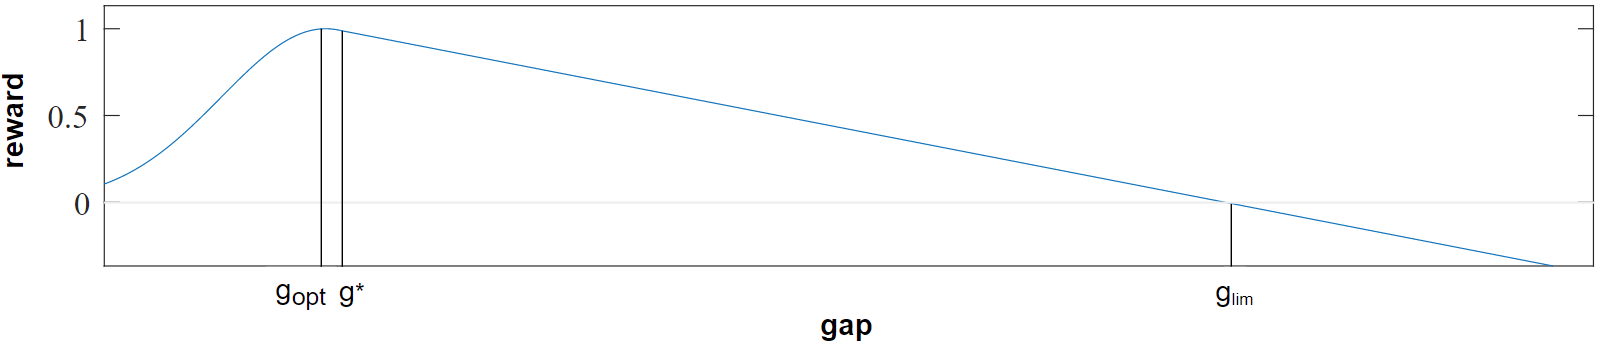
\includegraphics[width=12cm]{images/RewardFunc1}
	\caption{Reward function part 1 maximizes the reward for car following with time gap $T_{gap}$.}
	\label{fig:RewardFunc1}
\end{figure}


\begin{equation}
r_2 = 
\begin{cases}
\tanh\left(\frac{b_{kin}-b_{comf}}{a_{min}}\right),& \text{if } b_{kin}>b_{comf}\\
0,              & \text{otherwise}
\end{cases}
\end{equation}

with
\begin{equation}
b_{kin} = \frac{\Delta v^2}{s}
\end{equation}
The second part of the reward function addresses the vehicle behavior in safety-critical situations.
For a deceleration with the delay $b_{kin}$ the braking distance is equal to the current distance $s$. Thus, the kinematic deceleration $b_{kin}$ represents the minimum deceleration necessary to avoid a collision. A situation is considered as "safety-critical", if the kinematic deceleration $b_{kin}$ is greater than the comfortable deceleration $b_{comf}$. Thus, just in safety-critical situations the RL agent is getting penalized, illustrated in figure xy.

\begin{equation}
r_3 = -\left(\dfrac{da}{dt}\right)^2
\end{equation}

The third part of the reward function aims to reduce the jerk in order to achieve a comfortable driving. 

\begin{equation}
r_4 =  
\begin{cases} 
 -min\left(1,\left( v - v_{des}\right)^2\right), & \text{if } v>v_{des}\\
0, & \text{otherwise}
\end{cases}             
\end{equation}

The fourth part of the reward function penalizes the RL agent, if the current velocity $v$ is above the desired velocity $v_{des}$. 

\begin{equation}
r = 0.6r_1 + 1.1r_2 + 0.001 r_3 + r_4
\end{equation}

The weights of each reward part has been found experimentally and can further be optimized in future studies.

\subsection{RL algorithm}
In various similar control problems, the Deep Deterministic Policy Gradient (DDPG) Algorithm has been used and proven to perform well on tasks with a continuous action and state space (see xyz). In order to reduce the variance of policy gradients and increase learning speed, DDPG is an actor-critic method. The actor determines the action, while the critic judges about the quality of the action and how the policy should be adjusted. ([-> original paper DDPG])Both, actor and critic, are implemented as neural networks. In this study, both networks are feed-forward neural networks with two layers of hidden neurons and 32 neurons each hidden layer. All DDPG parameters are presented in Table \ref{tab:DDPGparameters}.

\begin{table}
	\caption{DDPG parameter values} 
	\label{tab:DDPGparameters} 
	\begin{center}
		\begin{tabular}{ p{0.4\textwidth} p{0.2\textwidth} }
			Parameter & Value \\ \hline
			Learning rate & 0.001 \\ 
			Reward discount factor & 0.95 \\ 
			Experience buffer length & 100000 \\ 
			Mini batch size & 32 \\ 			
			Gaussian noise mean & 0.15 \\ 
			Gaussian noise variance & 0.2 \\ 
			Gaussian noise variance decay  & 1e-5 \\ 
			Number of hidden layers & 2\\
			Neurons per hidden layer & 32\\
			

		\end{tabular}
	\end{center}
\end{table}


\subsection{Reward function}

learning input (leader speed time series)

[also relate parameters to driving style attributes such as desired
speed, accelerations, decelerations, desired time gap, minimum gap]


\section{Model training}
The training of the model comprises two important components, which have to be defined in advance. There is the generation of leading trajectories and the general definition of an training episode, that will be discussed in the following.

\subsection{Generating synthetic leading trajectories}
The leading trajectory is based on an AR(1) process, whose parameters reflect the kinematics of real leaders. The AR(1) process describes the speed of the Leader Vehicle and is defined as 

\begin{equation}
	v_l(t) = c+\phi v_l(t-1)+ \epsilon \text{, with } E(\epsilon) = 0, Var(\epsilon) = \sigma 
\end{equation}

With reaching of stationarity, this process has 
\begin{equation}
\label{eq:E_AR1}
 \text{an expected value of }E(v_l) = \frac{c}{1-\phi}, 
 \end{equation}
 
 \begin{equation}
 \label{eq:V_AR1}
 \text{the variance  }Var(v_l) = \frac{\sigma^2}{1-\phi^2}, 
 \end{equation}

 \begin{equation}
 \label{eq:ACF_AR1}
\text{the autocorrelation  }ACF(dt) = \phi^{dt}, 
\end{equation}

 \begin{equation}
 \label{eq:tau_AR1}
\text{and the correlation time  }\tau = -\frac{1}{ln(\phi)}, 
\end{equation}

with $d$ corresponding to the simulation step size, which is globally set to $100ms$. 

To adjust the parameters of the AR(1) process, typical values for real leader trajectories has to be defined: With $v_{l,des}$ as the desired velocity for the leader, the mean of the AR(1) process is set to be $v_{l,des}/2$ and the standard deviation is set to be $v_{l,des}$. The acceleration $a_{phys}$ corresponds to typical physical leader accelerations. With these values and by using Equation \ref{eq:E_AR1} - \ref{eq:tau_AR1}, the parameters of the AR(1) process can be calculated as:

 \begin{equation}
\phi = e^{(\frac{-2da_{phys}}{v_{l,des}})}
\end{equation}

 \begin{equation}
c=(1-\phi)\frac{v_{l,des}}{2}
\end{equation}

 \begin{equation}
 \sigma^2=(1-\phi^2)\frac{v_{l,des}^2}{4}
\end{equation}

The assumed typical values for $v_{l,des}$ and  $a_{phys}$ as well as the resulting values of the AR(1) process parameters can be found in Table \ref{tab:AR1Parameters}.

\begin{table}
	\caption{Assumed typical values for leading trajectories and the resulting values of the AR(1) process parameters} 
	\label{tab:AR1Parameters} 
	\begin{center}
		\begin{tabular}{ p{0.1\textwidth} p{0.1\textwidth} |p{0.1\textwidth} p{0.1\textwidth}  }
			 \multicolumn{2}{c|}{Real trajectory} & \multicolumn{2}{c}{AR(1) process}   \\ \hline
			$v_{l,des}$ &$15m/s$ &$\phi$ & $0.9933$\\
			$a_{phys}$ &$1m/s^2$ &$c$ & $0.05m/s$\\
			& & $\sigma^2$ & $0.75m^2/s^2$
			
		\end{tabular}
	\end{center}
\end{table}

Figure \ref{fig:AR1process} shows an example trajectory of the leading vehicle based on the AR(1) process using the parameters of Table \ref{tab:AR1Parameters}. If the velocity exceeds the defined range of $[0, v_{l,des}]$, it is manually set to the range limits.
\begin{figure}
	\centering
	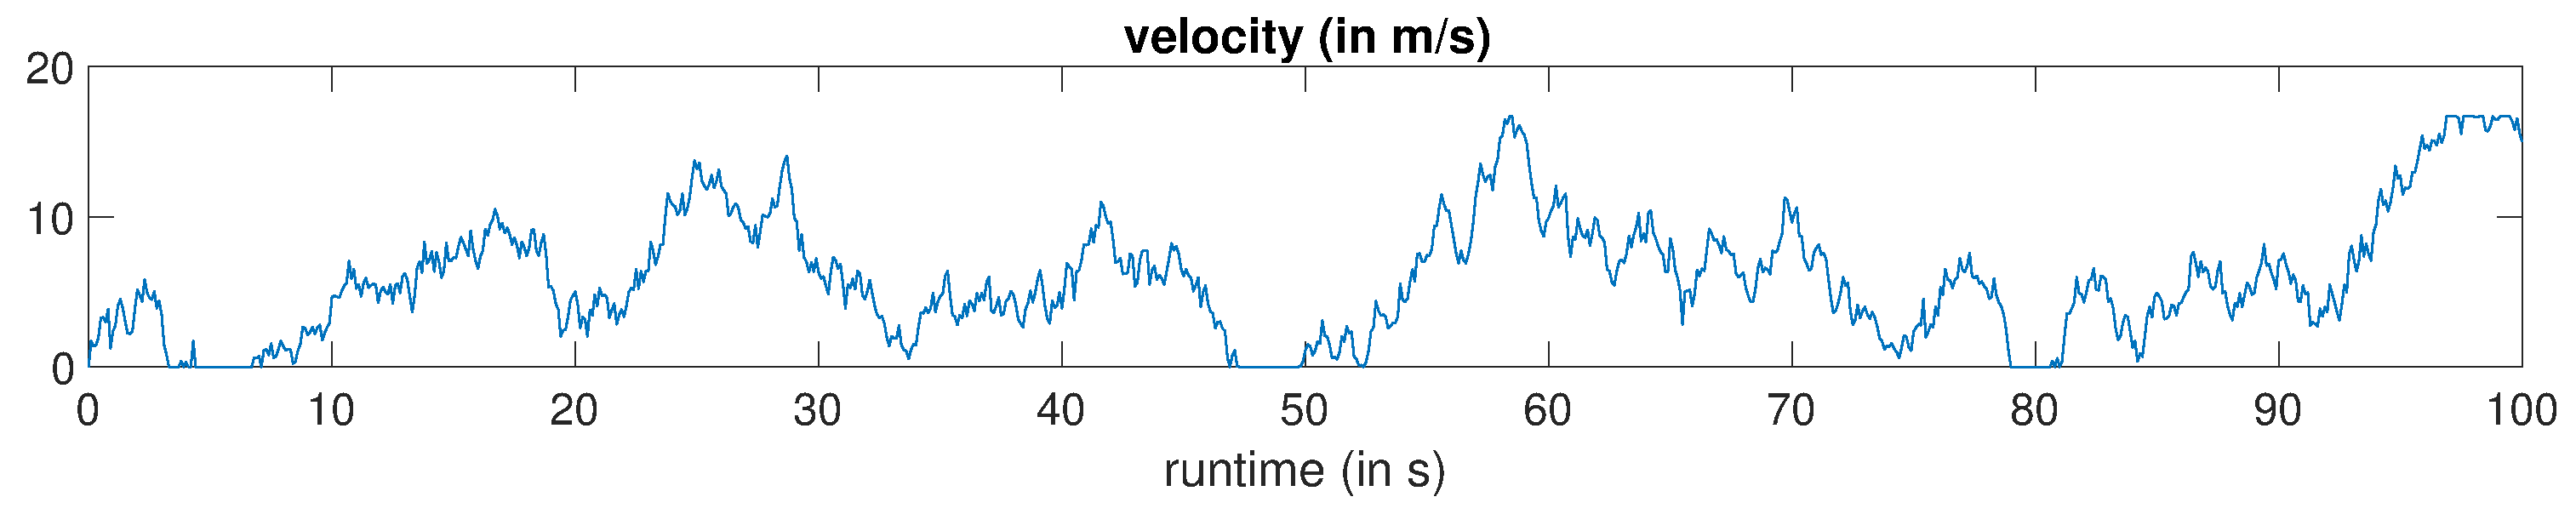
\includegraphics[width=0.95\textwidth]{images/AR1process}
	\caption{Example of a leading trajectory based on the parametrized AR1 process used to train the RL agent}
	\label{fig:AR1process}
\end{figure}


\begin{figure}
	\centering
	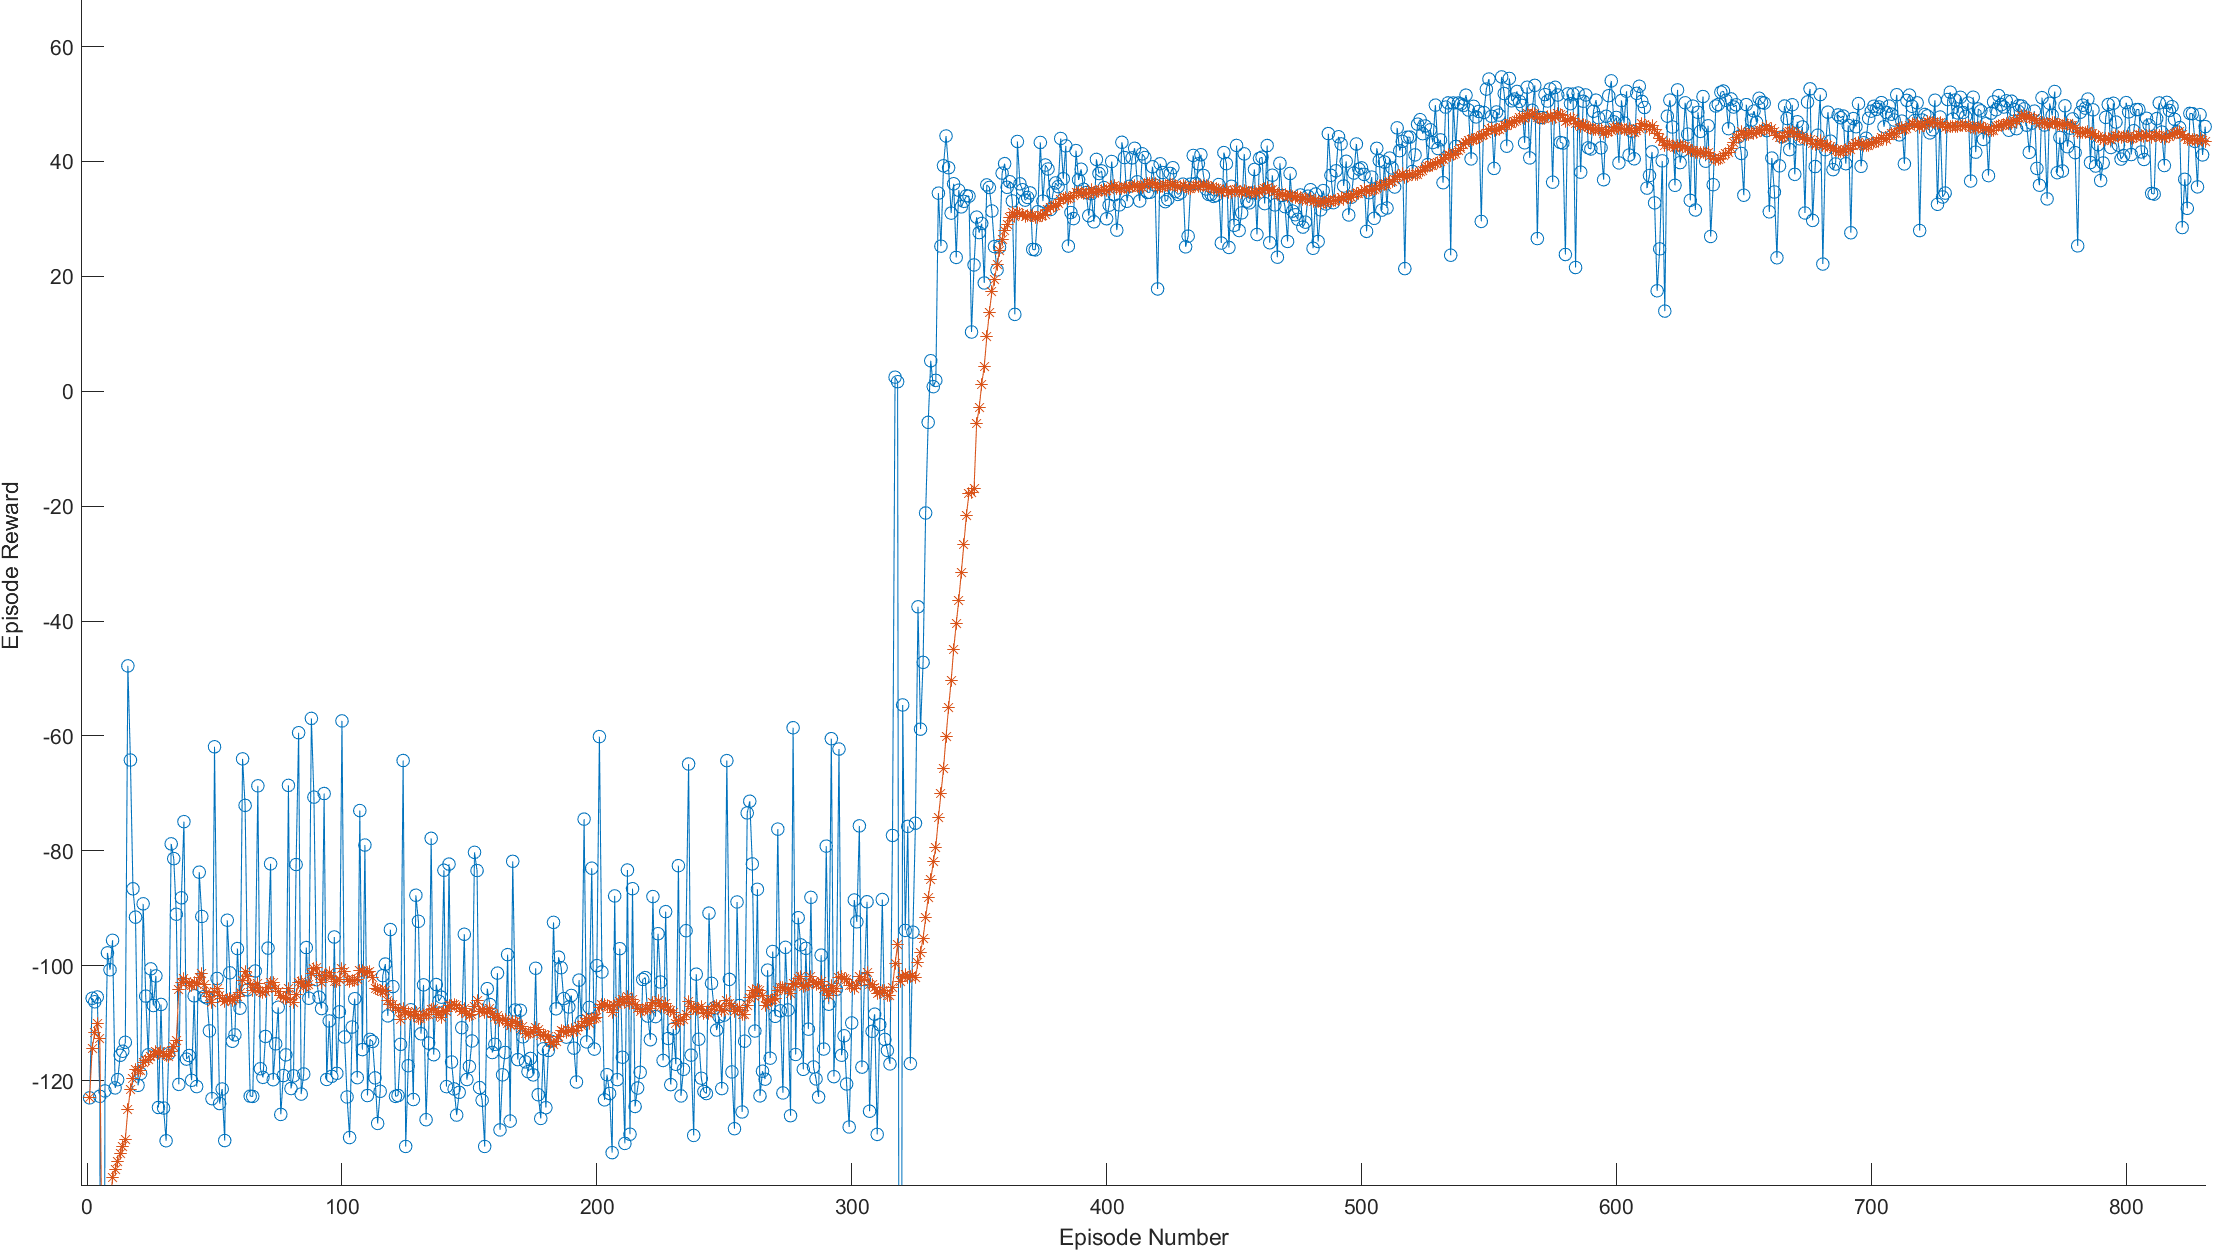
\includegraphics[width=0.95\textwidth]{images/Training}
	\caption{RL training process, one episode containing 500 steps}
	\label{fig:training}
\end{figure}

\subsection{Training episode definition}

To train the RL agent, a training episode has to be defined. One episode has a simulation time of $50s$ with a step size of $d=100ms$, resulting in a episode length of $500$ steps. The initial velocities of Follower and Leader Vehicle is a randomly set in the range $[0,v_{des}]$ respectively  $[0,v_{l,des}]$. The initial gap between both is set to $120m$. 

\subsection{Results of the RL training process}

Figure \ref{fig:training} shows an example of the training process. The red line shows the moving average reward of the last 30 episodes. After approximately 570 episodes the maximum average reward has been reached. Reaching saturation the learning process has been stopped after 850 episodes. 

\section{Validation}

The goal is not to minimize some error measure as in usual
calibration/validation but to check if the driving style is safe,
effective, and comfortable. The RL strategy is evaluated with respect to these metrics in different driving scenarios, described in the following.

\subsection{Response to an external leading vehicle speed profile}
The first scenario is designed in order to evaluate the transition between free driving and car-following as well as the Follower behavior in safety-critical situations. 
Figure \ref{fig:manipulatedLeader} shows a driving scenario with an external Leading Vehicle speed profile. The initial gap between Follower and Leader is 200 meters, which refers to a free driving scenario. The Follower accelerates with $a_{max} = 2m/s^2$ until the desired speed $v_{des} = 16.6m/s$ is reached and approaches the standing Leader Vehicle. When the gap between both drops below 90 meters, the Follower starts to decelerate with a approximately $b_{comf} = -2m/s^2$ (transition between free driving and car-following) and comes to a standstill with a final gap of approximately $s_{min} = 2m$. In the following the Leader Vehicle makes some random acceleration and deceleration. At the time $t = 40s$ the Leading Vehicle makes a full brake, resulting in a comfortable and safe braking of the Follower Vehicle. The transition between different accelerations happens in a comfortable way, reducing the resulting jerk. 



\begin{figure}
	\centering
	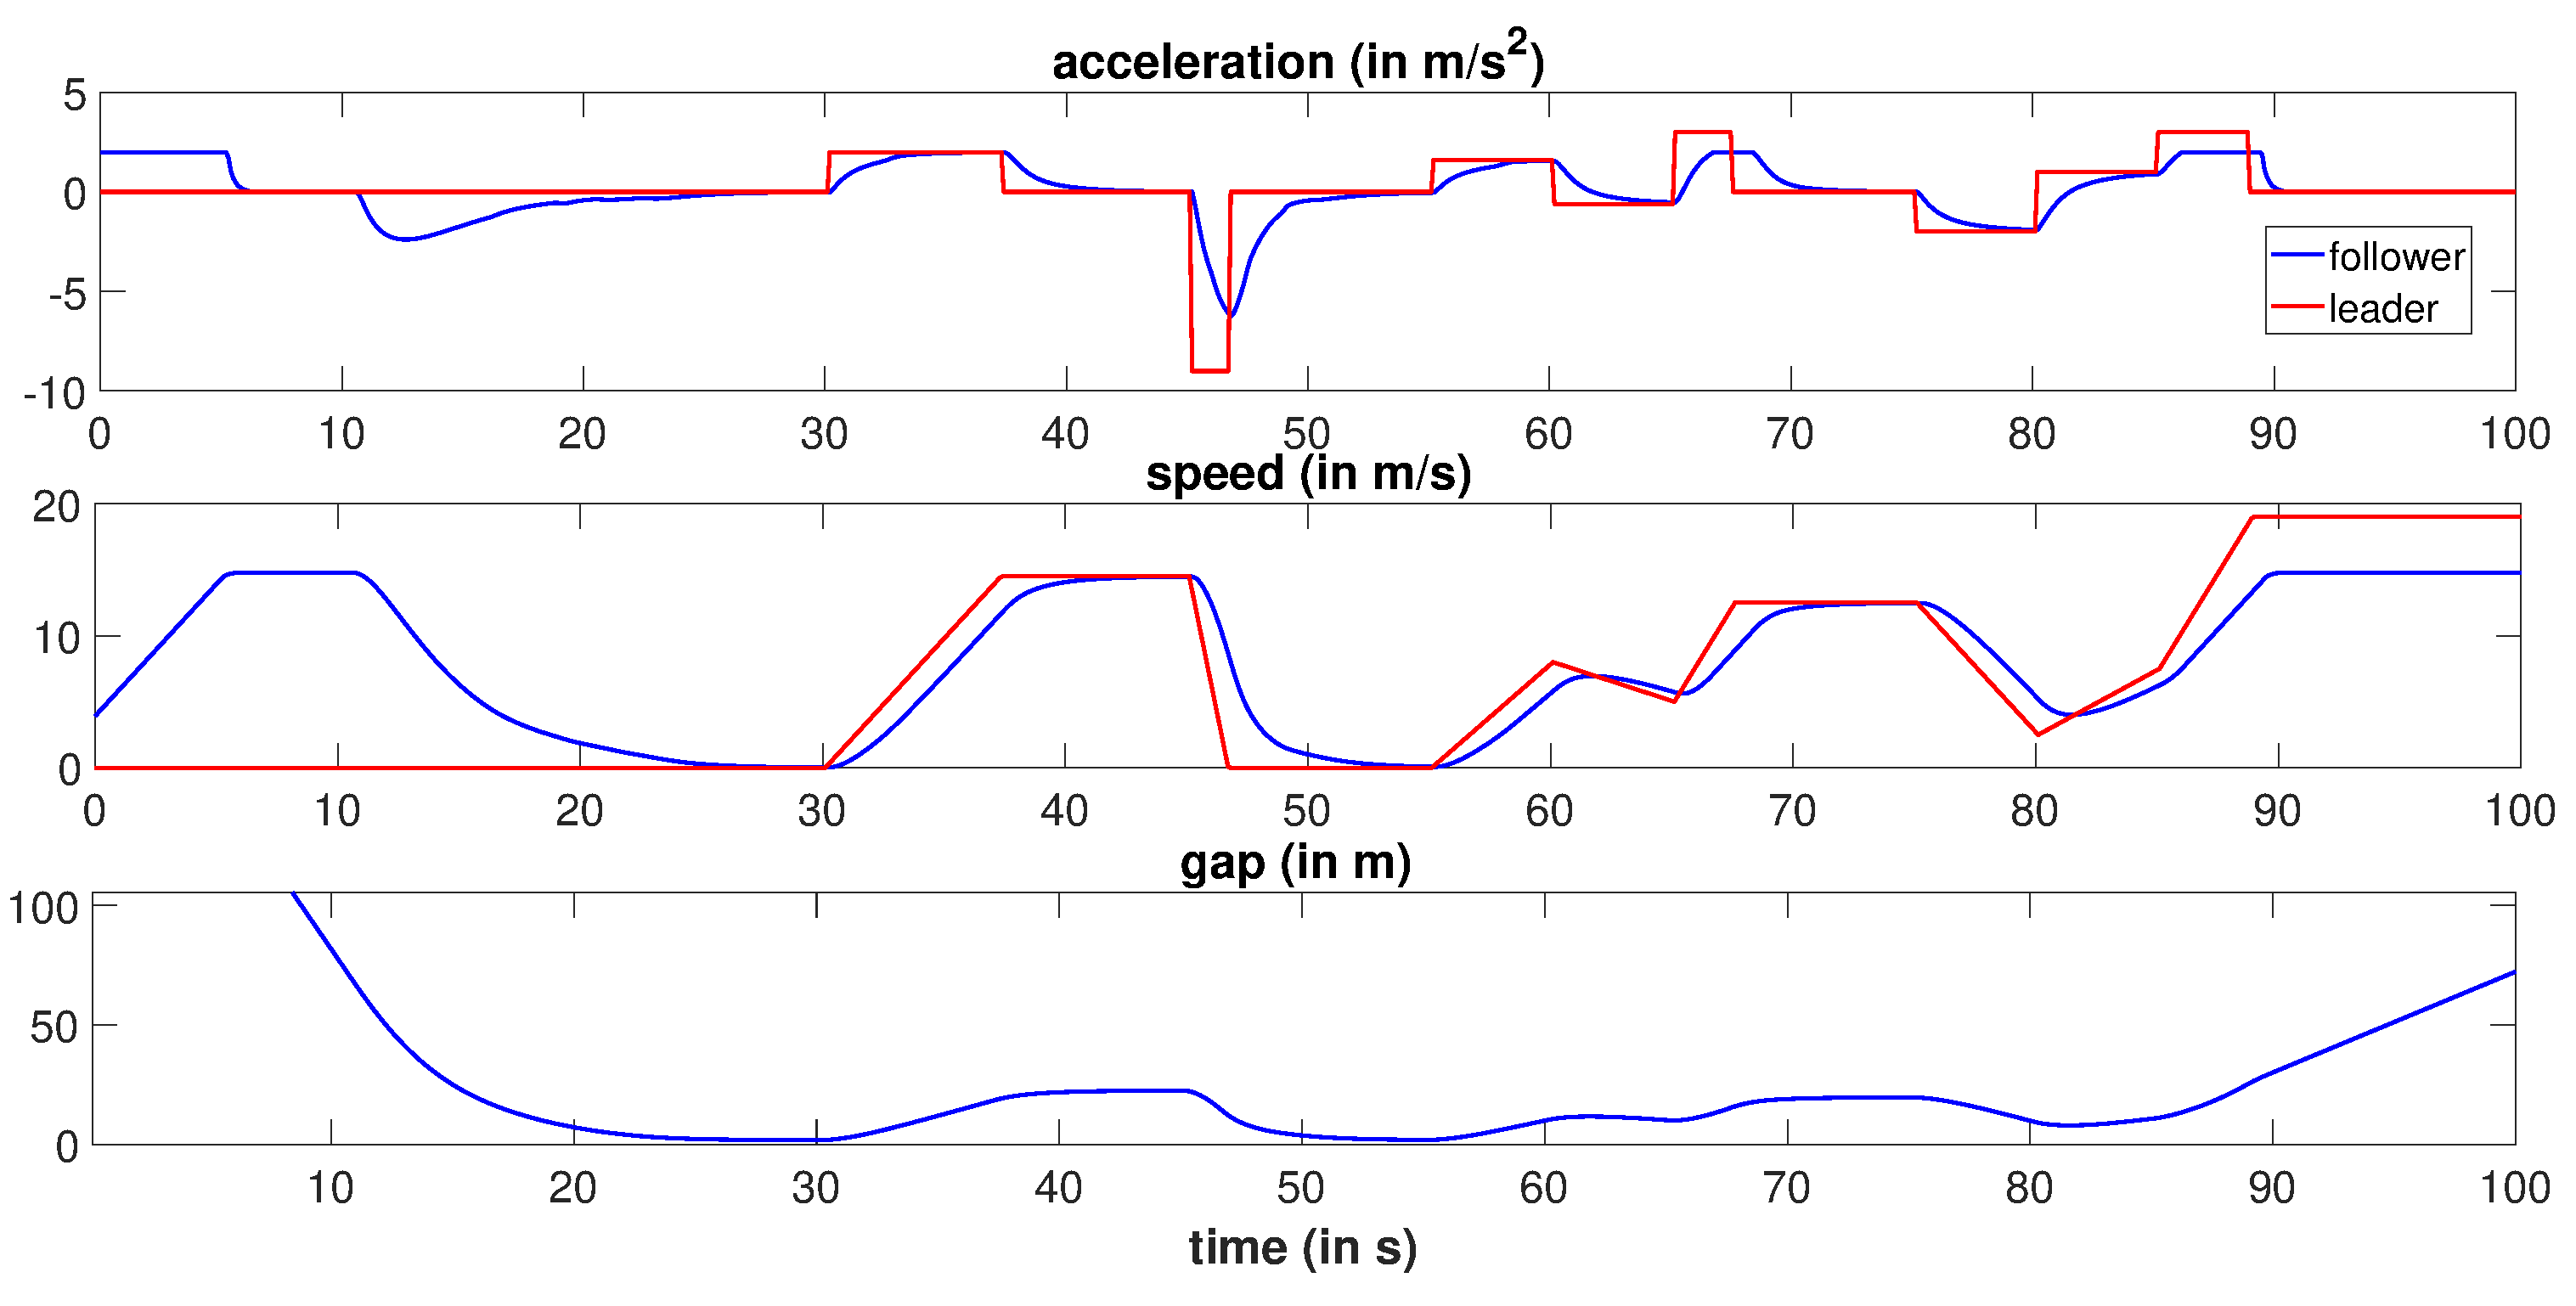
\includegraphics[width=0.95\textwidth]{images/manipulatedLeader.eps}
	\caption{Response to an external leading vehicle speed profile}
	\label{fig:manipulatedLeader}
\end{figure}

\begin{figure}
	\centering
	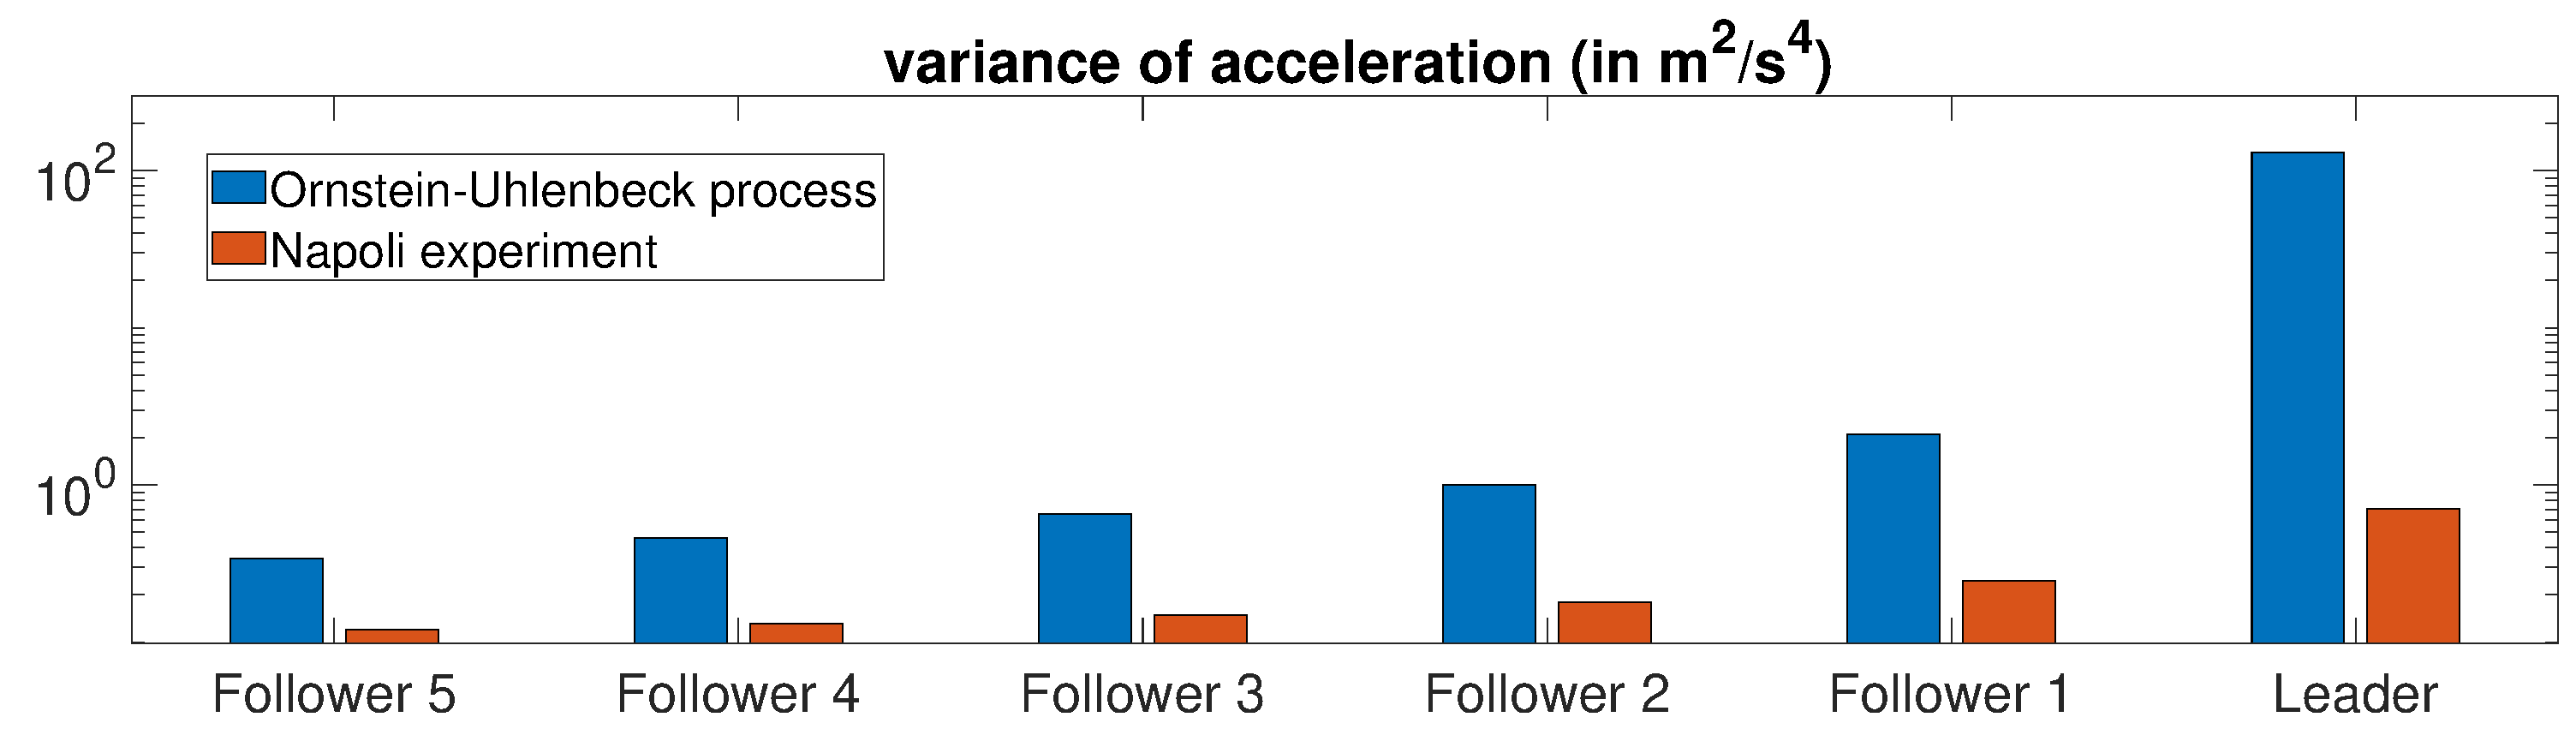
\includegraphics[width=0.95\textwidth]{images/VarAccComp}
	\caption{Comparison of the acceleration variance between Leader and Follower for AR(1) and Napoli experiment}
	\label{fig:VarAccComp}
\end{figure}






\subsection{String stability}
\label{sec:stringStability}
The second scenario, shown in Figure \ref{fig:AR1Kolonne}, consists of a Leader based on the AR(1) process, followed by five vehicles, each controlled by the trained RL agent. The results show that traffic oscillations can effectively be dampened with a sequence of trained Followers, even if the Leader shows large outliers in acceleration. Figure \ref{fig:VarAccComp} illustrates the difference of accelerations between Leader and the Followers (blue bars). The last Follower shows the lowest variance of acceleration, which demonstrates the ability of the RL agent to flatten the speed profile, to dampen oscillations and thus to increase comfort.  


\begin{figure}
	\centering
	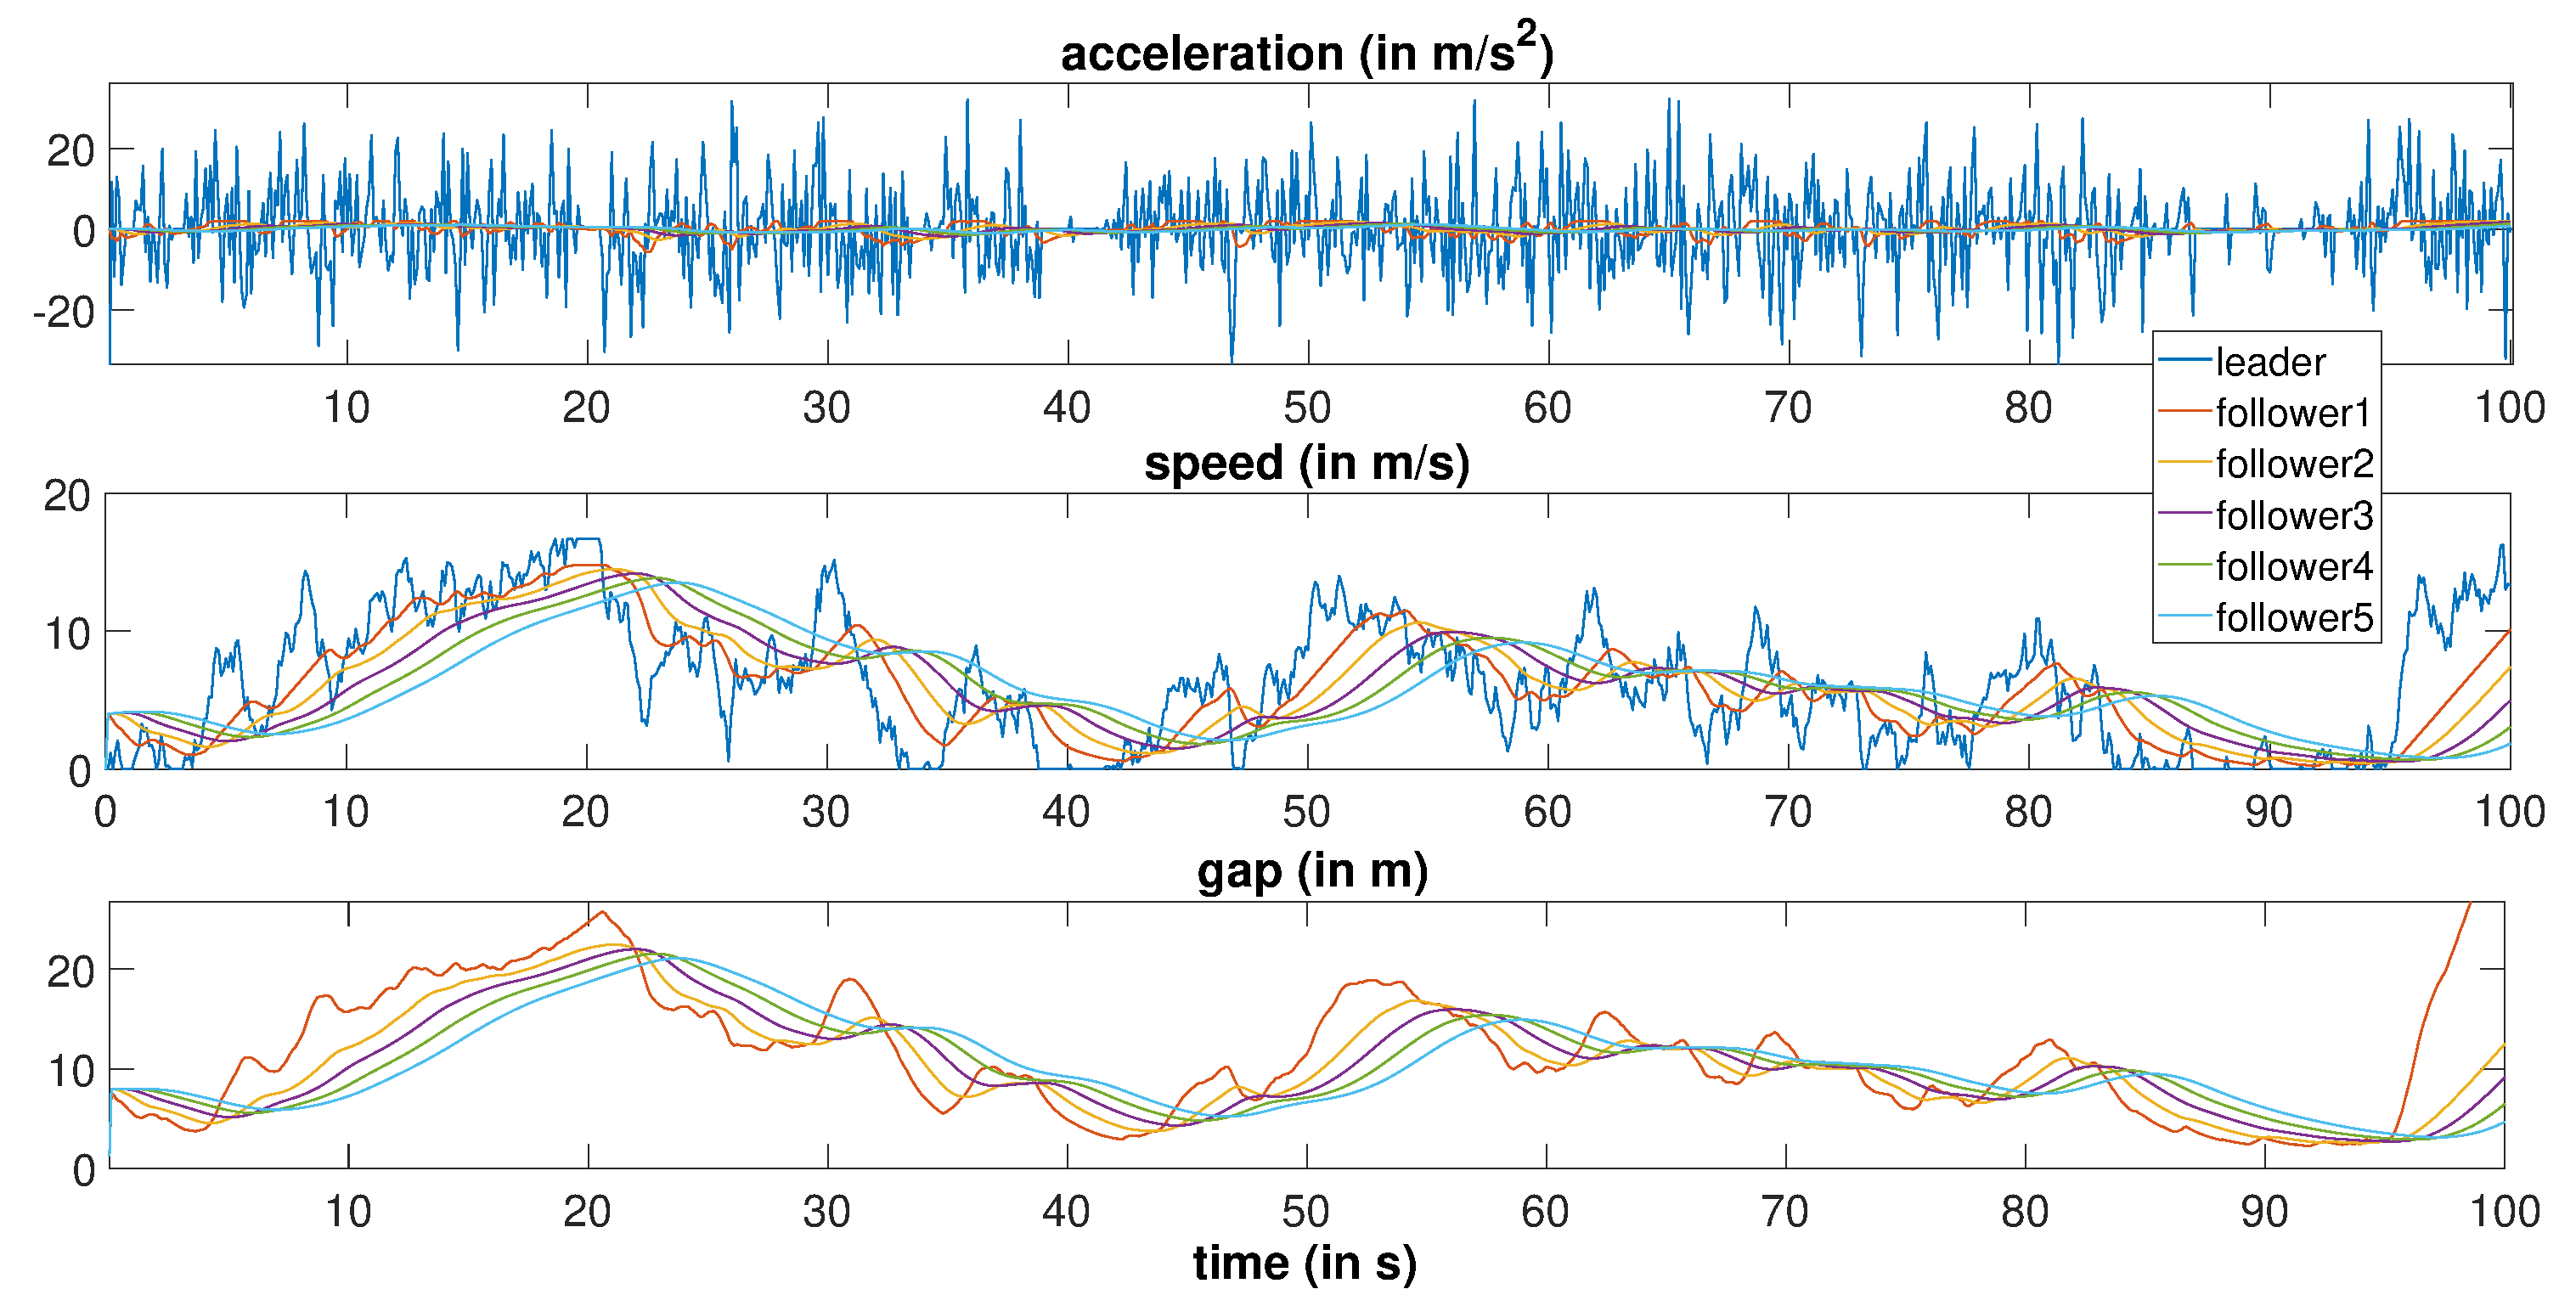
\includegraphics[width=0.95\textwidth]{images/AR1Kolonne}
	\caption{Response to a leader trajectory based on a AR(1) process}
	\label{fig:AR1Kolonne}
\end{figure}


\subsection{Response to a real leader trajectory}

In a further scenario, the abilities of the RL strategy are evaluated with a real leader trajectory. This trajectory comes from experiments in Napoli, where exact data from Leader and Follower were obtained (reference to Punzo et al.). Figure \ref{fig:PunzoKolonne} shows the result of a sequence of five vehicles following a real leader trajectory. Similar to the experiment from Section \ref{sec:stringStability} string stability and the reduction of acceleration variance, shown by the red bars in Figure \ref{fig:VarAccComp}, is demonstrated. At time $t = 140s$ the Leader stands still, and it can be observed, that all following vehicles are keeping the minimum distance $s_{min}$ to the Leader. 


\begin{figure}
	\centering
	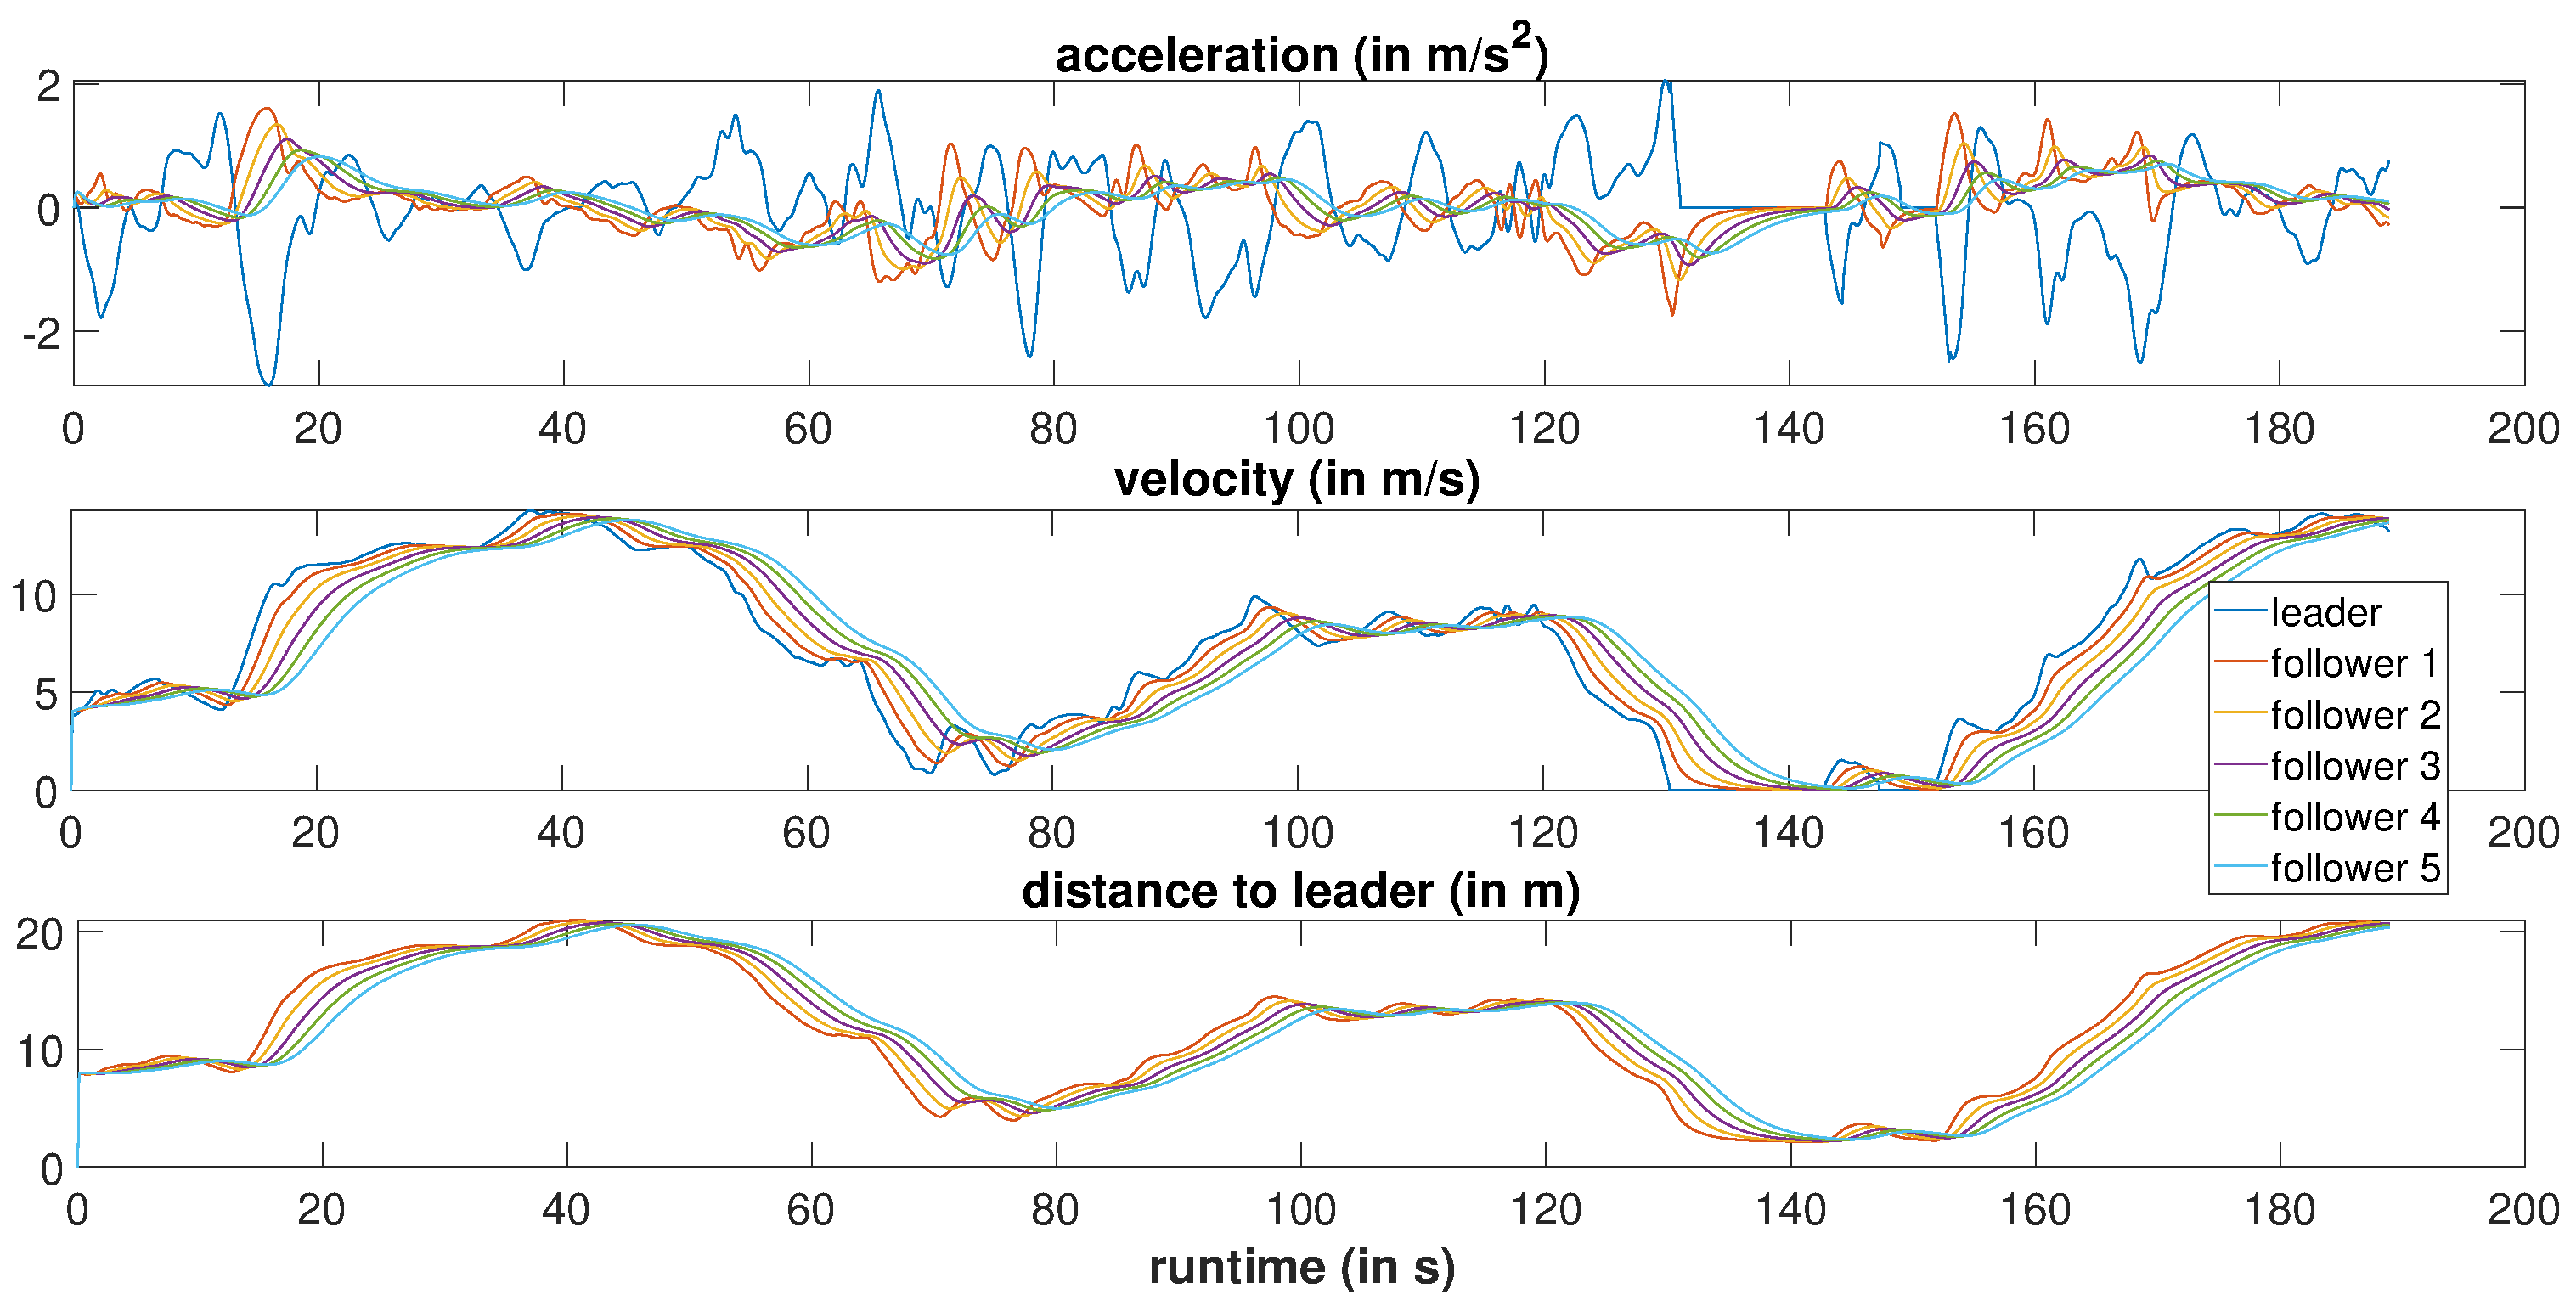
\includegraphics[width=0.95\textwidth]{images/PunzoKolonne}
	\caption{Response to a real leader trajectory}
	\label{fig:PunzoKolonne}
\end{figure}


\subsection{Response of different driver characteristics}
\label{sec:differentT}

As mentioned in Section \ref{rewardFunction}, different driving styles can be achieved by adjusting the parameters of the reward function. Three RL agents has been trained on a reward function, that differs in the desired time gap $T_{gap}$ between Follower and Leader Vehicle ($T_{gap,1} = 1.0s$, $T_{gap,2} = 1.5s$, $T_{gap,3} = 2.0s$). Figure \ref{fig:differentT} shows the result of these agents, following the real leader trajectory from Napoli. It can be observed, that a lower value for $T_{gap}$ results in closer driving to the Leader, higher accelerations and decelerations and thus in a more aggressive driving behavior. 

\begin{figure}
	\centering
	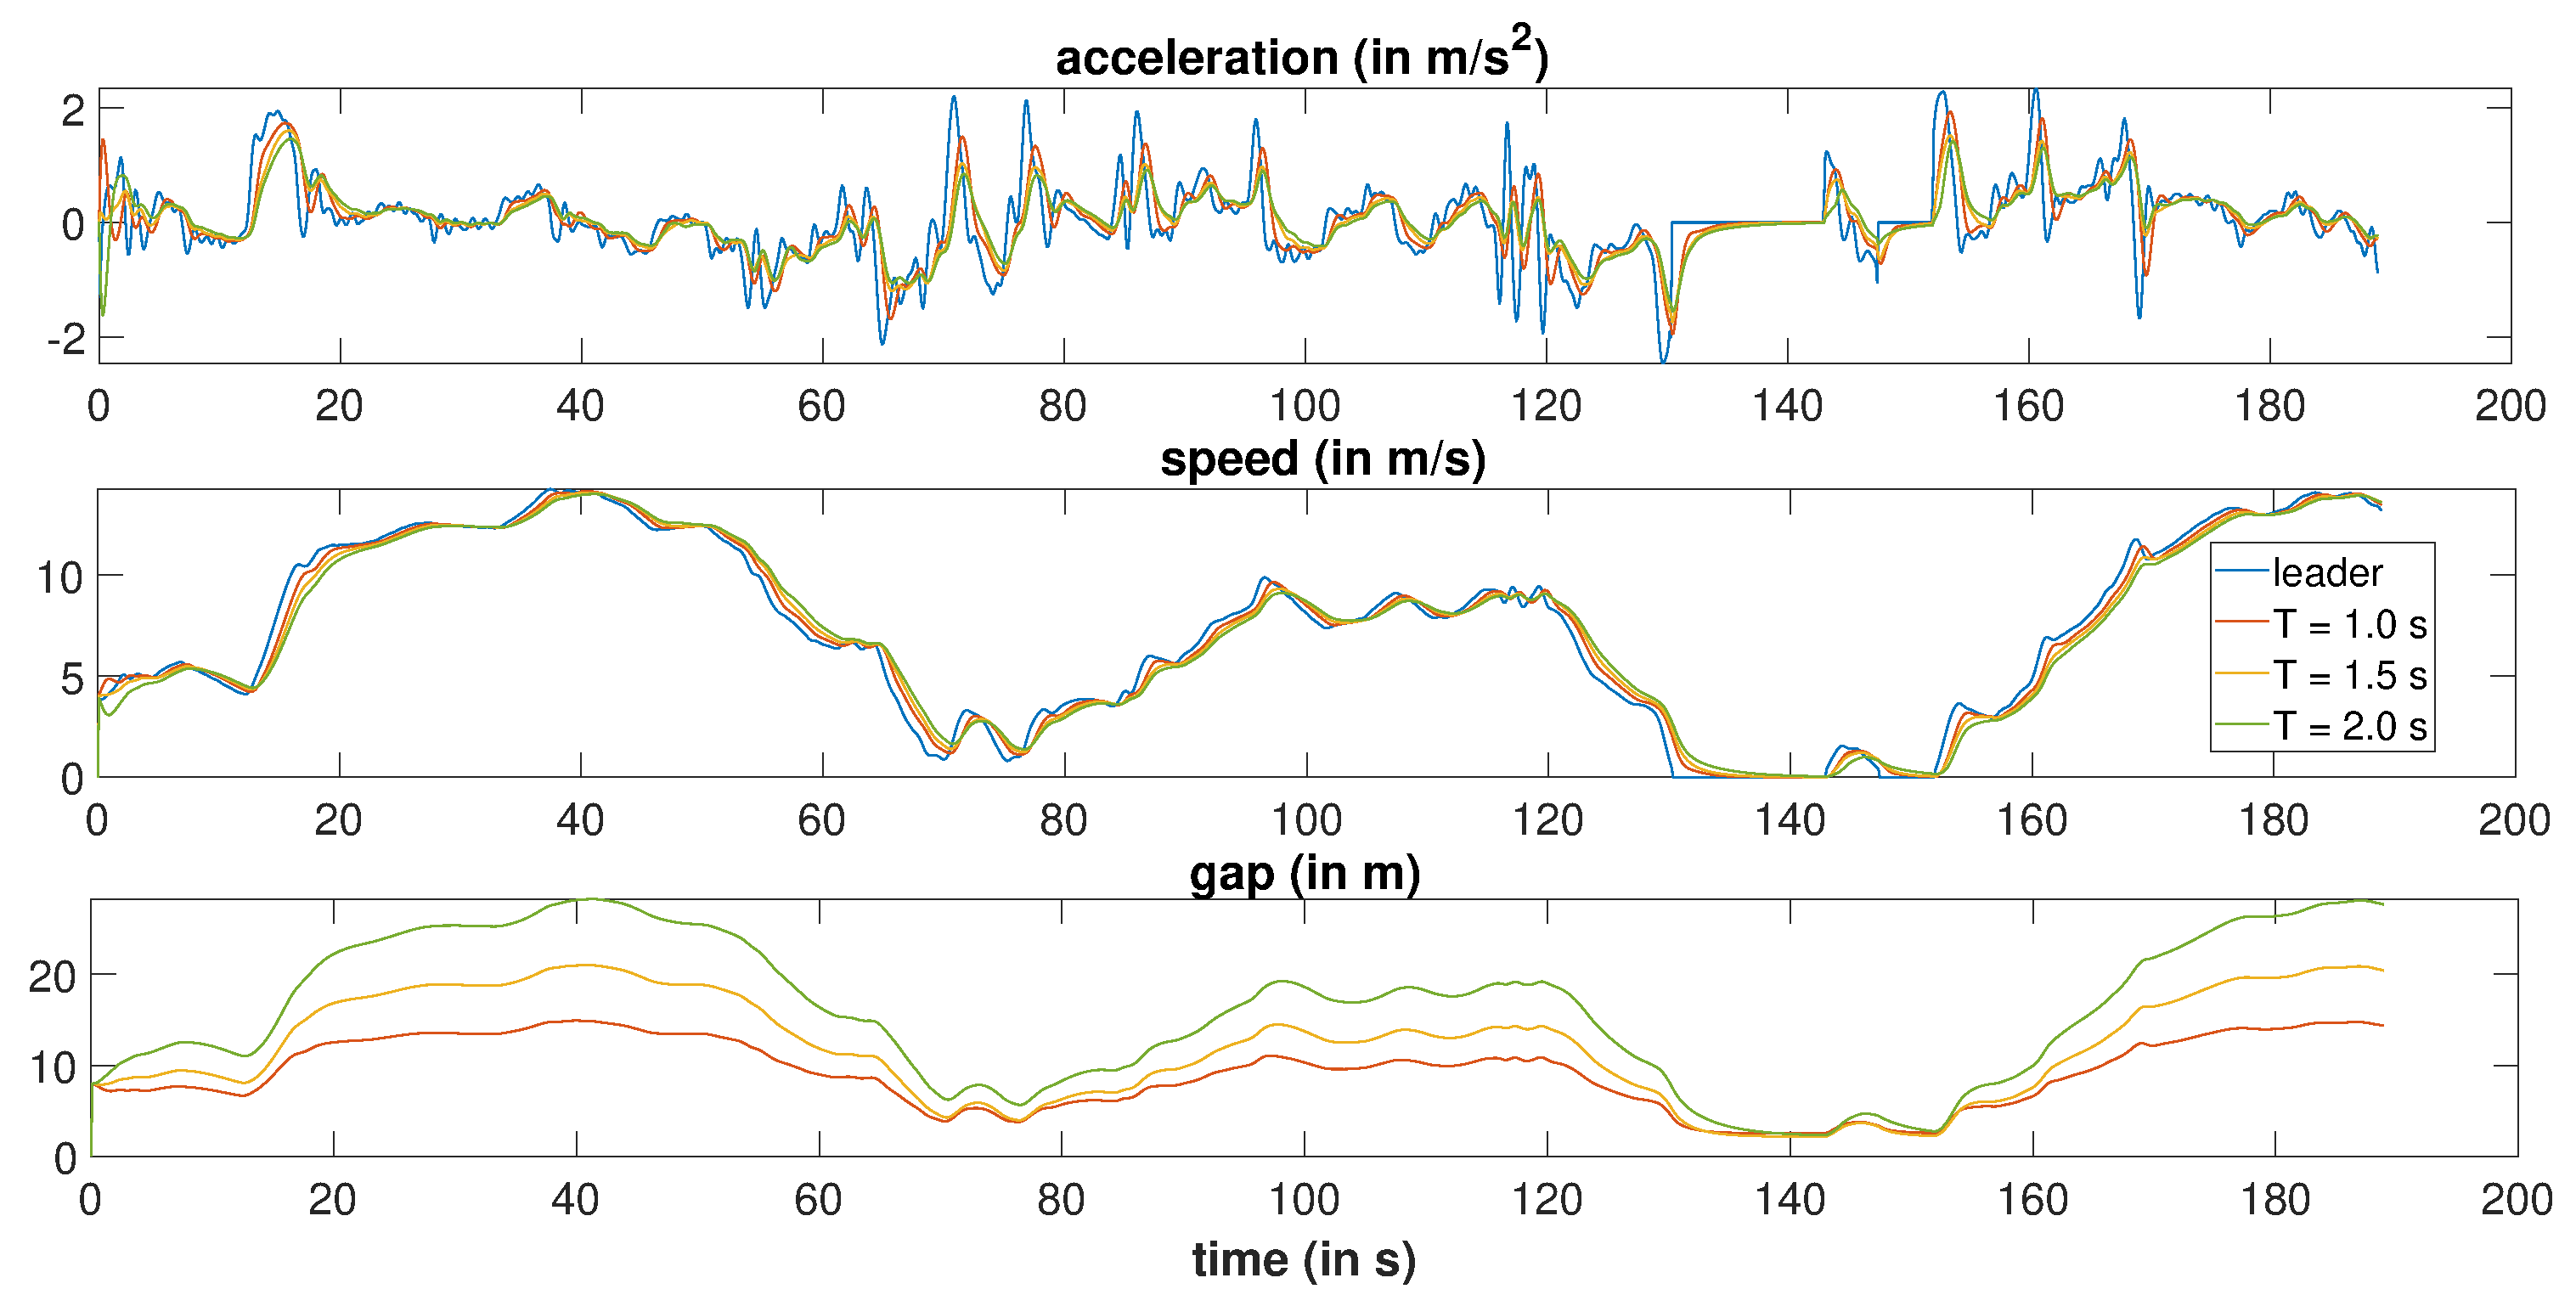
\includegraphics[width=0.95\textwidth]{images/differentT}
	\caption{Impact of different parametrized RL agents on driving behavior}
	\label{fig:differentT}
\end{figure}


\section{Conclusion/Discussion}
evaluation of safety and comfort, comparison to IDM

discussion: adjusting parameters of the reward function to achieve different driving styles

\section*{References}

\bibliography{RL_vehicles_references}

\end{document}
